\chapter{Task 1}
% TODO How is the element notated graphically or textually
\section{UML Model elements}
All the visual notation for the elements listed below are present in this picture:
\begin{figure}[hbt]
\label{Class}
  \centering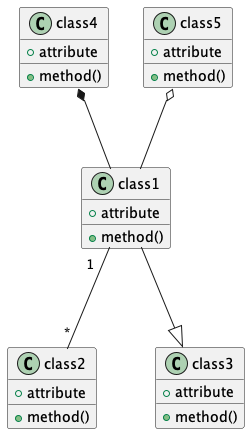
\includegraphics[width=0.4\textwidth]{Immagini/test-3.png}
  \caption{Class}
\end{figure}


\subsection{Class}
The purpose of a class is to specify a classification and the Features of objects and to define their structure and behaviour. The structure and behaviour of objects is characterised by classes, and classes can act as a namespaces for other classes defined within their scope. A class is shown using the Classifier symbol : the default notation for a classifier is a solid outlined rectangle with the classifiers name, with compartments separated by horizontal lines below the name, the name should be centered and in boldface, and should begin with a uppercase letter.If the class is abstract it is written in italics. Compartments can be supressed and then seperator lines aren't drawn and no inference may be drawn from the presence or abscence of the elements in the supressed compartments. A Class has four mandatory compartments: attributes operations receptions and internal structure (and these must appear in this order). If the class represents a meta class may be extended with <<Metaclass>> before its name. And a class can have optional compartments that all classifiers can have. Any compartment that contains features may show these grouped under the strings: private public protected representing their visibility. A compartments name may be shown or hidden it should be centered and start with lowercase letters, it can contain spaces but no punctuation. A class with the property isActive = true can be shown by a class box with an extra vertical line on each side. Any keywords including stereotype names can also be written centered in plain face in a pair of "<<" above the name of the class name if there are multiple keywords/stereotypes then each enclosed in a separate pair of << and listed one after the other or listed all in the same pair of << separated be commas.
\subsection{Objects}
Instance specifications represent the possible or actual existence of an instance in a modeled system and completely or partially describe these. Instace Specifications represent instances of Classifiers and Classes are classifieres in a modeled system. InstanceSpecifications are depicted like classifiers with the exception that in the place where the Classifier name is written, the name of the instance followed by a colon followed by the classifier names if any (and if there are multiple then these are separated by commas) is written and underlined. Names are Optional for Classifiers and InstanceSpecifications, the standard name for an unnamed Classifier or anonymous Instance Specification is an underlined colon, If the Instance Specification has Value specifications these are represented with: value name followed by "=" followed by a value-specification in the enclosing shape. Structural features if any are shown with structural feature name followed by = followed by a value specification. There aren't any mandatory parts except maybe that the box with the name need to be drawn.\\
 An object has a well-defined boundary and is meaningful in the application. Objects have these characteristics:
\begin{itemize}
	\item State $\rightarrow$ The state is the condition in which an object can exist. An object’s state is implemented with a set of attributes and usually changes over time.
	\item Behavior $\rightarrow$ Behaviour determines how an object responds to requests from other objects. Behaviour is implemented by a set of operations.
	\item Identity $\rightarrow$ The identity of an object makes it unique. You can use the unique identity of an object to differentiate between multiple instances of a class if each instance has the same state.
\end{itemize}
Each object must have a unique name. A complete object name has three parts: object name, role name, and class name. You can use any combination of the parts when you name an object. The following table shows several object name variations for an online shopping system. 
\begin{figure}[hbt]
\label{object}
  \centering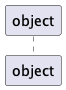
\includegraphics{Immagini/test-2.png}
  \caption{Object}
\end{figure}

\subsection{Attribute}
Properties Represent attributes of classifiers, a member of an Association or both, they also represent attributes of Classes since they are classifiers. Properties are represented as a string consisting of the visibility followed by / followed by the name : followed by the property type followed be the multiplicity type in "[" brackets, followed by "=" followed be the default value followed by any modifiers in "{" brackets. In Classifiers the type visibility , default , multiplicity and proprietary string may be suppressed from being displayed even if the values are in the model. Properties can be shown in columns rather than continuous strings. And an attribute may be shown using the association notation where the hollow or filled diamond is shown at the end of the tail. There aren't really any mandatory
\subsection{Operation}
An Operation is a behavioural feature of a class, datatype or interface. Operation elements specify the name type, Parameters and Constraints for When These Operations are Invoked (Executed) on instance of their Featuring Classifiers. An Operation is a Feature of a Class and determines what its objects can do and how. Operations are shown with text stings in the form of:[<visibility>] <name> ‘(‘ [<parameter-list>] ‘)’ [‘:’ [<return-type>] [‘[‘ <multiplicity-range> ‘]’] [‘{‘ <oper-property> [‘,’ <oper-property>]* ‘}’]]. Operations probably must be shown in this form it seems everything is optional except the name + "()".

\subsection{Associations}
An association describes a semantic dependency between two classes. The semantics dependency can range from simple message passing to enclosing one class within another. The details of the semantic dependency may not be explicit in the diagram.\\

 Each association may optionally have a label. Though unnamed associations are somewhat vague for the designers and implementers, UML does not require a label for an association. If present, the label of an association uniquely determines the association itself.\\ 
 
 An association is generally uni-directional; the direction of the association is implied by the meaning of the label; so, the designer is expected to choose a suitable name for the association that is meaningful in the current application.\\
 
 An arrow is attached to the association label or to one end of the association in order to indicate the direction explicit.\\
 
 An association must connect exactly two classes; it is possible for an association to connect the same class on either end in which case it is called a recursive association.\\
 
  There can be any number of distinct associations between the same pair of classes. An association may optionally have a cardinality on either end of the association. A cardinality symbol (also called multiplicity in UML) is of the form 'n..m' where n and m are numbers, n >= 0, m >= 0 and m >= n.\\
  
  When an association from a class A to B has a cardinality of n..m at the end close to the class B, it is read as "every object of class A is associated with n to m objects of class B at the same time". The symbol '*' can also be used in place of 'n..m', which means 'zero or more'.\\
  
  An association may optionally have a role. A role symbol is a label close to the participating class. Consequently, each class in the association may have a role.\\
  An association may optionally have one or more constraints enclosed in curly brackets and placed near the association. Sometimes, the constraints may be imposed on more than one association. 
\subsection{Multiplicity}
A Multiplicity Element is an Element that can be instantiated to represent a collection of values depending on the type of element. Associations can have multiplicities.The notation is specified for each type of Multiplicity element but in general a notation will be shown as a text string containing the bounds of the multiplicity and a notation for showing the optional ordering and uniqueness specifications.It can also be displayed as a symbol. A multiplicity can be shown in the format <lower-bound>..<upper-bound> .Just at least Some notation about a bound is required if there is one. Further optional Components depend on the specific Multiplicity element.
\subsection{Generalisation}
Generalisation elements depict a relationship in which a (child) element is based on another (parent) element. This is used to indicate that for example: in class diagrams child classes receive all attributes operations and relationships defined in their parent class. A generalisation Relationship is represented as a solid line with a hollow arrowhead that points from the child element to the parent element placed at the end of the line at the parent element. At least this is required it seems. The lines can be named to designate generalisation Sets with names written near the line, two lines to the same parent can be joined so that they are part of the same generalisation set.
\subsection{Aggregation}
 An aggregation relationship between a pair of classes indicates that an object of one class encloses an object of the other class. The class at the diamond end of the aggregation symbol is an aggregate and the other class is a component. For example, the class "Polygon" aggregates the class "Line", in which case the diamond end of the aggregation symbol must touch the class "Polygon". An aggregation is also an association; however, there are some differences. The representation of an aggregation is: a solid line with an unfilled diamond at the association end which is connected to the classifier that represents the aggregate.
\subsection{Composition}
A Composition Association Relationship represents a relation ship where An element is comprised of another, and that the life time of the part classifier is dependent on that of the whole classifier. Classifiers can be composed of other classifiers so Classes can be composed of other classes so they would have such a relationship depicted between them. A composition association relationship depicted with a solid line with and a filled diamond at the association/end of the line which is connted to the whole/composite classifier.